\chapter{Mise en \oe{}uvre}
\section{Ouverture}
\paragraph{}
Dans ce chapitre, nous présenterons l'architecture globale de notre système ainsi que notre hypothèse et la structure de l'application que nous avons développée pour concrétiser cette hypothèse. La dernière partie de cette section porte sur les résultats de cette étude.
\section{Analyse des Besoins}
\paragraph{}
Le large succès de Wikipedia (qui est le 6ème site le plus visité sur internet selon le classement de google en mais $2012$, des $1000$ sites les plus visités au monde\footnote{http://www.neodia.fr/apprendre/13-etudier/364-les-1000-sites-les-plus-visites-selon-google}) et le progrès des techniques d’extraction des données ont abouti à la naissance et la construction automatique  de larges bases de connaissances comme DBpedia, YAGO, etc.
\subparagraph{}
Beaucoup de connaissances sont construites en se basant sur l’extraction automatique des faits relationnels à partir de ces sources d'informations.
En effet, les bases de connaissances convergent sur les faits statiques et ne donnent pas une grande importance à la dimension temporelle de ces triplets.
En dépit du fait que la majorité des faits évoluent avec le temps, ou ne sont valides que dans une période temporelle précise. Ainsi, nous remarquons que le temps a une dimension significative dans ces bases de connaissances.
\subparagraph{}
La dimension temporelle est particulièrement importante dans les relations binaires comme $isPresidentOf$, $isCEOof$, $isMarriedTo$. Une base de connaissances contenant plusieurs présidents des États-Unis ne peut être consistante que lorsqu’on ajoute une dimension temporelle à ces faits. De plus l’annotation temporelle aide à faire la distinction entre les faits courants et les faits dépassés.
Par exemple le fait ``Kennedy est le président des États-Unis'' est correct, mais n'est plus valide.
Lorsqu’on attache une annotation temporelle à un fait comme celui là, il devient universellement valide.
\section{Étude préliminaire et approches possibles}
\subsection{Web Collaboratif}
\paragraph{}
Le Web collaboratif est le Web qui s'appuie sur les utilisateurs pour construire son contenu. Nous avons commencé notre travail de recherche par une étude préliminaire autour du contenu de ces plateformes collaboratives. Aussi, nous avons étudié les pistes possibles pour l'exploitation des sauvegardes Wikipédia et Wikidata. Tout d'abord, nous avons téléchargé les fichiers des collections XML et nous avons observé la structure des informations dans ces sources d'informations. Ensuite nous avons implémenté un premier algorithme d'extraction en utilisant un parseur XML (SAX\footnote{http://www.saxproject.org/}).
La figure ci-dessous représente notre schéma de modélisation dans lequel nous avons procédé avec une modélisation qui touche directement les sources principales d'informations Wikipédia et Wikidata.
\begin{figure}[H]
        \centering
                \centering
                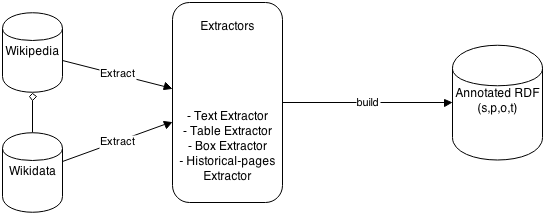
\includegraphics[width=13cm]{modelisation.png}
               \caption{Première approche : schéma de modélisation générale}

\end{figure}
\subparagraph{}
Cette modélisation est une première rubrique d'analyse et de conception d'une solution qui touche les besoins préliminaires de notre étude. Par ailleurs, nous avons retrouvé une autre modélisation plus proche de nos besoins principaux et que nous détaillerons par la suite.
\subsection{Notre proposition}
\paragraph{}
En analysant les $dumps$ DBpedia et en observant l'architecture de cette base de connaissances, nous avons remarqué que pour annoter temporellement les triplets RDF de DBpedia il est plus intéressant d'extraire l'ensemble des propriétés dans DBpedia c'est-à-dire : nous utilisons directement les données de DBpdedia au lieu de mettre en place des nouveaux extracteurs à partir des sources Wikipédia, puis de trouver des faits qui ont trait au temps, donner une liste de couples à partir de laquelle un expert choisit un couple et valide les résultats de notre algorithme.
\subsection{Modélisation}
\paragraph{}
Le modèle quaternaire est un modèle qui représente la base RDF d'un fait précis et le fait rattaché au premier ayant une dimension temporelle. Les deux exemples suivant montrent le principe de ce modèle.
\begin{verbatim}
f1:<politician, elected, president of US>
f2:<politician, happenedDate, date>

f1, Kennedy elected PresidentOf USA 
f2, Kennedy happenedDate 08/11/1960

f1:f2, <Kennedy, elected, presidentOf USA, 08/11/1960>

f1,f2 Kennedy elected PresidentOf USA happenedDate 08/11/1960
\end{verbatim}
$HappenedDate$ est utilisée pour dire que le fait est valide que dans ce point du temps, équivalente à tempProp de notre système.
\paragraph{}
{\it Pour les faits valides que dans un intervalle de temps , nous avons la représentation suivante:}
\begin{verbatim}
<politician, servedAs, politicianOffice, from startedOnDate 
to endedOnDate>
\end{verbatim}
\begin{figure}[H]
        \centering
                \centering
                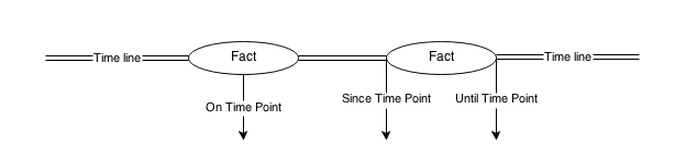
\includegraphics[width=13cm]{timeline.png}
               \caption{Chronologie des événements}

\end{figure}
\subparagraph{}
Ce modèle est capable d'exprimer la validité temporelle d’un triplet RDF d’une manière à la fois structurée et lisible par la machine. On s'intéresse particulièrement au format N-Quads comme format de sortie de notre algorithme.
\subsection{Notre hypothèse}
\paragraph{}
Après une observation approfondie dans les sources de données dans DBpedia, nous avons repéré des relations entre des propriétés comme \{($firstAssent$-
$Person$, $firstAssentYear$) ou ($beatifiedBy$, $beatifiedDate$)\}. Nous avons trouvé plusieurs propriétés qui ont un lien logique entre elles, les relations temporelles ont comme objet un point du temps particulier et partagent le même sujet ou la même ressource avec une autre propriété.
\subparagraph{}
Durant cette étude nous avons essayé de valider cette hypothèse :
\begin{verbatim}
if (x tempProp t) and (x relatedProp z) then
             (x relatedProp z) t 
\end{verbatim}

\begin{itemize}
\item $tempProp$ est une propriété DBpedia dont le nom contient un préfixe temporel ($Year$, $Date$).
\item $relatedProp$ est une propriété DBpedia avec un nom qui a le même suffixe.
\end{itemize}
$t$ est l'annotation temporelle du triplet ($x$,$relatedProp$,$z$).
\subparagraph{}
Nous avons présenté cette hypothèse sous forme d'une requête SPARQL. Cette requête interroge l'ensemble des ressources sur DBpedia et retourne des résultats si c'est possible.
Notre hypothèse porte principalement sur le fait d'annoter temporellement les ressources de DBpedia en essayant de repérer deux triplets portant sur un même sujet et permettant de les relier dont le but est d'avoir un quadruplet valide. La liste des couples ($tempProp$, $relatedProp$)
est donnée comme sortie d'une procédure d'extraction de l'ensemble des propriétés de DBpedia. Toutefois, cette procédure n'est pas automatique, elle nécessite un validation de la part d'un expert.
\section{Outils de développement}
\subsection{ Java}
\paragraph{}
Le choix de développer le logiciel sous forme d'une application $Java$ était un choix personnel et qui s'explique de nombreuses manières. Premièrement, la maîtrise de ce langage de programmation me permet d'utiliser des différentes structures de données et d'explorer la documentation de certaines méthodes plus facilement. De plus, il existe plusieurs sources de documentation sur le Web. En outre une large communauté aide à répondre aux questions si jamais on rencontre des difficultés. Il existe une version Java de DBpedia et cela permet plus facilement d'intégrer mon application open source et disponible sur mon compte\footnote{https://github.com/metanote/Extraction} github. Enfin, nous avons utilisé les librairies $ApacheJena$ qui sont aussi écrites en Java. 
\subsection{Jena}
Aparche Jena\footnote{https://jena.apache.org/} est un $Framework$ open source écrit en Java pour construire des applications dans les domaines du
$LinkedData$ et le Web sémantique. Nous avons utilisé les différentes librairies des ce $Framework$ pour interroger DBpedia avec des requêtes SPARQL. $Jena$ est composé de plusieurs programmes différents qui interagissent entre eux pour traiter des données écrites en RDF. $Jena$ fournit un support pour le langage de définition d'ontologies (OWL). Ce $Framework$ se compose des différentes API RDF, Ontology et SPARQL, une couche interface d'application et une troisième couche pour le stockage. La figure\footnote{http://jena.apache.org/getting\_started/} ci-dessous présente en détaille les différentes composantes de Jena.
\section{Contribution}
\subsection{Architecture du système}
 \begin{figure}[H]
        \centering
                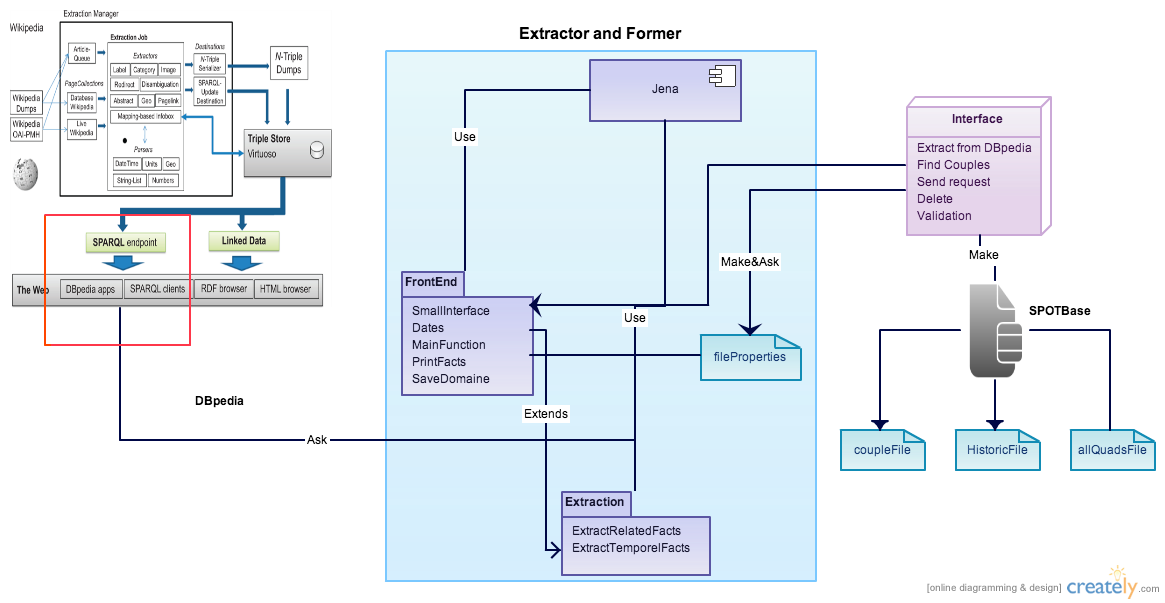
\includegraphics[width=16cm]{NEWArchitecture.png}
               \caption{Architecture de l'application}
\end{figure}
\paragraph{}
L'architecture de notre application se repose principalement sur celle de DBpedia et plus précisément, nous utilisons le point d'accès SPARQL. En premier lieu, nous interrogeons DBpedia pour avoir une liste de propriétés. En effet, nous pouvons prendre la liste de toutes les propriétés en interrogant DBpedia en utilisant les librairies Jena sous Eclipse avec la requête \begin{verbatim} select distinct ?P where {?S ?P ?O},\end{verbatim}mais on se limite aux propriétés de DBpedia qui ont la forme suivante \begin{verbatim} ?S rdfs:domain ?O \end{verbatim} $rdfs{:}domain$ est une instance de $rdf{:}Property$ qui est utilisé pour indiquer que toute ressource qui possède une propriété donnée est une instance d'une ou plusieurs classes. Le triplet précédant indique que, $S$ est une instance de la classe $rdf{:}Property$, $O$ est une instance de la classe $rdfs{:}Class$ et les ressources désignées par les sujets des triplets dont le prédicat est $S$ sont des instances de la classe $O$. Lorsque une propriété $S$ a plus d'une propriété $rdfs{:}domain$, les ressources indiquées par les sujets des triplets avec prédicat $S$ sont des instances de toutes les classes indiquées par les propriétés $rdfs{:}domain$. $rdfs{:}domain$ peut être appliqués à lui-même. $rdfs{:}domain$ de $rdfs{:}domain$ est la classe $rdf{:}Property$. Cela veut dire que toute ressource avec une propriété $rdfs{:}domain$ est une instance de $rdf{:}Property$. 
\subparagraph{}
Ensuite, nous avons choisi de stocker l'ensemble des propriétés dans un fichier ``fileProperties'' pour ne pas avoir des contraintes de mémoire (stockage dans la mémoire vive à chaque fois) et pour ne pas interroger la base de connaissances à chaque fois. Cette procédure se fait une seule fois lors du premier lancement de l'application et elle ne sera plus nécessaire après, car il suffit de spécifier le nom du fichier des propriétés DBpedia que nous avons utilisé lors de la première exécution, mais nous avons mis la possibilité d'extraction et mise à jour de ce fichier parce qu'il se trouve que DBpedia change et il y a des propriétés qui s'ajoutent au fur et à mesure à cette base de connaissance. Puis, à partir de ces propriétés, nous avons implémenté un algorithme d'extraction qui produit en sortie une liste de couples de propriétés ($tempProp$, $relatedProp$). Dans l'application, nous avons choisi de prendre l'avis d'un expert pour valider les résultats de notre algorithme à travers une liste labellisée d'une partie des quadruplets que nous avons réussi à former et à extraire automatiquement dans un $output$ $Textarea$. Nous avons écrit notre hypothèse de base sous forme d'une requête SPARQL de la manière suivante :
\begin{verbatim}
PREFIX rdfs: <http://www.w3.org/2000/01/rdf-schema#> 
PREFIX dbp:<http://dbpedia.org/ontology/> 
SELECT CONCAT(?label1, relatedProp , ?label2, ' : ', ?date) 
			WHERE {  
					 ?S   		dbp:relatedProp 	 ?O;
							dbp:tempProp		 ?date;
							rdfs:label 			 ?label1.
					?O 		rdfs:label ?label2.
					FILTER(lang(?label1)='en' && lang(?label2)='en'}
\end{verbatim}
{\it - tempProp est une propriété temporelle proposée.}
\newline
{\it - relatedProp est une propriété reliée à tempProp partage avec elle un même suffixe.}
\subparagraph{}
L'objectif de cette procédure est de permettre à l'expert de valider ou ne pas valider la logique de la représentation des quadruplets. Enfin, la validation des résultats permet de stocker l'ensemble des résultats (triplets annotés) dans un fichier portant les labels du couple et dans un autre fichier ``allQuadsFile'' contenant tous les quadruplets validés. Par la suite, un sauvegarde de l'historique de cette procédure se fait automatiquement dans le fichier CSV. Ce fichier nous permet d'avoir une vision globale sur les résultats de notre étude. $historic.csv$ a la forme suivante :
\newline
{\tt (relatedProp,tempProp,boolean,exploration\_Date,keep,file)} 
\begin{itemize}
\item $relatedProp$ et $tempProp$ représentent le couple de propriétés DBpedia.
\item $boolean$ peut être $0$ ou $1$ qui désignent respectivement la volonté de l'expert de valider ou ne pas validé les résultats.
\item $exploration\_Date$ est la date de l'exploration.
\item $keep$ représente le nombre de quadruplets que nous avons formé à partir d'un couple de propriétés.
\item $file$ est le nom de fichier dans lequel nous avons stocké les résultats (Quadruplets) relatifs à chaque couple.
\end{itemize}
\newpage
\subsection{Analyse et discussion}
\paragraph{}
Nous avons réussi à former $305$ couples de propriétés. Dans notre méthode, nous avons choisi d'extraire même les couples ($tempProp$, $relatedProp$) qui contiennent un motif similaire de la forme suivante (tempProp, ***suffixeTempProp***) et non pas seulement qui sont identiques au suffixe d'une propriété temporelle. Cela a été dans la mesure d'augmenter le nombre des couples de propriétés de test pour avoir une vision globale sur l'efficacité de notre système, d'avoir plus de possibilités et d'analyser par la suite les différents résultats. 
Avec certains couples, nous avons eu de très bons résultats, par exemple avec le couple ($deathCause$,$deathYear$) nous avons réussi à formé $2766$ quadruplets. La figure ci-dessous montre le format de la sortie de notre algorithme.
 \begin{figure}[H]
        \centering
                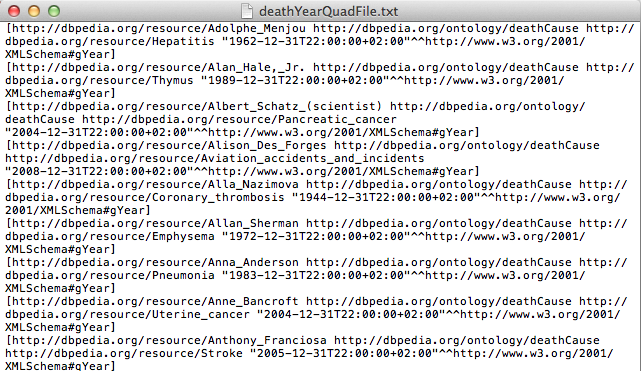
\includegraphics[width=15cm]{DeathYearCause.png}
               \caption{Fichier de Quadruplet DeathYear et DeathCause}
\end{figure}
\subparagraph{}
Il se trouve aussi qu'il y a des couples qui valident notre hypothèse mais qui ne donnent pas de résultats. Il se peut que les deux triplets ne partagent pas le même sujet comme \{(wineRegion, wineYear),(whaDraft, whaDraftYear),(areaCode, areaDate), etc.\}
\subsection{Résultats et Exploration}
\paragraph{}
Durant cette étude, nous avons réussi à former automatiquement un nombre important de quadruplets à partir de couples de propriétés qui valident notre hypothèse. Pour donner des résultats, notre programme prend des temps d'exécution variés qui ne dépassent pas trois minutes, selon le nombre des quadruplets extraits, pour donner des résultats. Sachant qu'on utilise une machine sous OS x avec un processeur $2$ GHz Intel Core i$7$ et $8$ GO de mémoire. Parmis nos meilleurs résultat celle du couple de propriétés (BirthPlace, BirthDate) donnent $814~514$ triplets annotés. Nous avons stocké plus que $988~051$ quads que nous avons réussi à former dans le fichier $AllQaudsFile$. Nous avons remarqué que certains couples valident bien notre hypothèse et donne des excellents résultats. Certes, il y a d'autres couples ne donnent aucun résultat. Le problème, c'est que toutes les propriétés DBpedia ne suivent pas toujours la même logique de représentation. Si tel n'était pas le cas, nous pouvons avoir beaucoup plus de résultats.
\subparagraph{}
Dans toute l'exploration des résultats extraits, nous appellerons couple significatif, le couple ($tempProp$, $relatedProp$) juger comme intéressant par l'expert et éventuellement si l'extraction à travers la requête SPARQL fournit des résultats significatifs. Nous avons utilisé le logiciel  RStudio\footnote{http://www.rstudio.com/products/rstudio/release-notes/} pour le traitement et d'analyse statistique de données de $historic.csv$, le tableau ci-dessous présente une partie du contenu de ce fichier. 
 \begin{figure}[H]
        \centering
                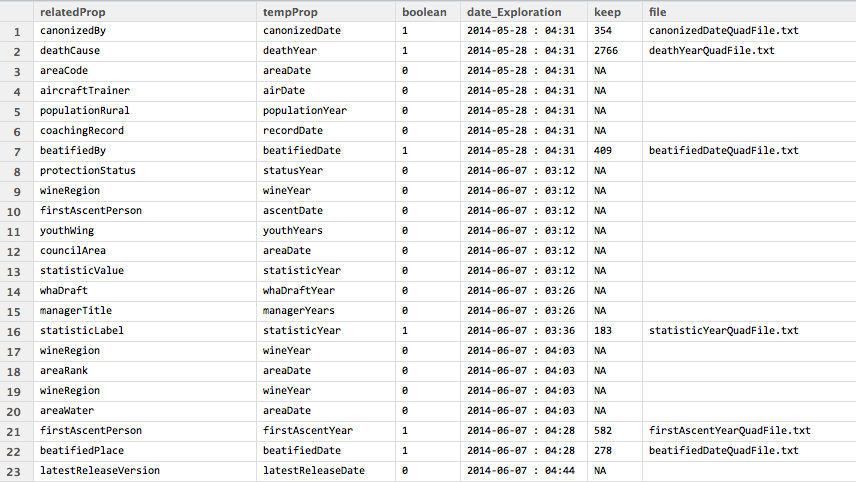
\includegraphics[width=13cm]{tableauCSV.png}
\end{figure}
Les diagrammes (figure 2.5 et figure 2.6) présentent des statistiques sur les résultats de notre système d'extraction.
Nous avons $70$ données explorées soit $22,9$\% du nombre totale de couples extraits, chaque observation porte sur (deux noms de propriétés RDF, une valeur boolean oui/non intéressant, date d'exploration, nombre de t-uples et le nom de fichier de sauvegarde).
\begin{itemize}
\item Le nombre de couples non-significatifs : $44$ parmi les $70$ couples explorés.
\item Le nombre de couples significatifs :  $26$ parmi les $70$ couples explorés.
\item Le porcenatage de couples significatifs est de $37,1429$\%.
\item Les valeuers de frequence rencontrées sont entre $0$ et $814~514$.

\end{itemize}
 \begin{figure}[H]
        \centering
                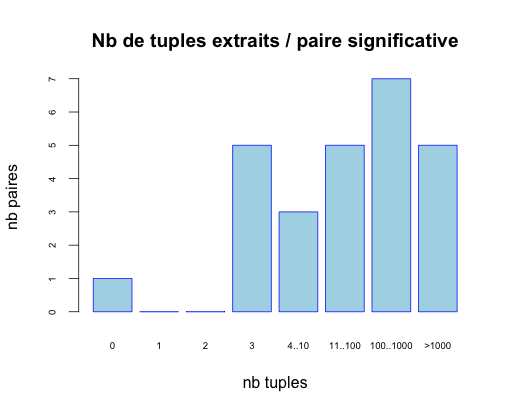
\includegraphics[width=11cm]{dessin1.png}
               \caption{Histogramme du nombres de tuples extraits par une paire jugée comme significative}
\end{figure}

\begin{figure}[H]
        \centering
                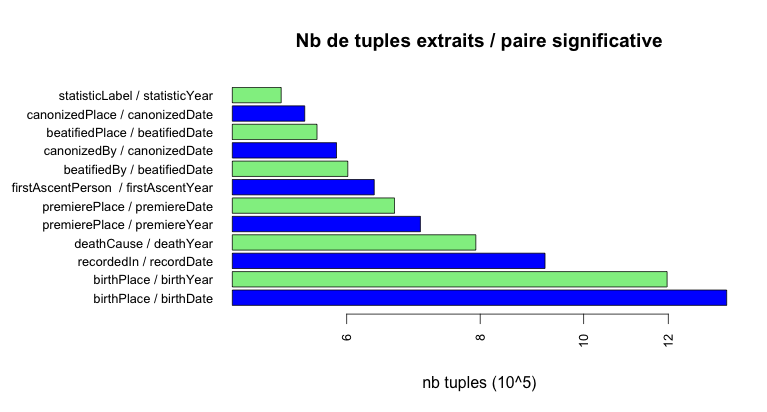
\includegraphics[width=12cm]{dessin2.png}
               \caption{Diagramme des paires significatives ayant plus de $100$ tuples extrais (l'échelle est log-logarithmique)}
\end{figure}
\subparagraph{}
Dans la figure ci-dessus, on indique uniquement les couples ($relatedProp$, $tempProp$) qui générent plus de $100$ quadruplets.
\subsection{Réflexions}
\paragraph{}
Dans le Web sémantique, nous avons remarqué qu'il est très important de mettre des conventions pour la représentation des données. Cela permet non seulement d'utiliser les triplets existants, mais aussi de mettre des hypothèses permettant de construire des travaux au dessus de ce qui existait. Le Web sémantique évolue s'il se repose sur une structure de métadonnées générique, claire et réutilisable. Dans cette étude, nous avons traité des triplets DBpedia. Nous avons réussi à implémenter une solution pour annoter des triplets qui ont trait au temps et nous avons mis ces triplets sous la forme quadruplets. Nous avons manipulé une partie de triplets de la base de données d'entrée pour construire notre base de données quadruplets de sortie $SPOTBase$. La représentation de connaissances sous forme de triplets, nous permet non seulement de les réutiliser dans des divers types de traitements, mais aussi de faire des déductions à partir de ces triplets pour exprimer d'autres concepts. 
